\documentclass[addpoints]{exam}
\usepackage{amsmath, amsfonts, amssymb}
\usepackage{geometry}
\usepackage{hyperref}
\usepackage{titling}
\usepackage{forest}
\usepackage{titling}
\usepackage{tikz} % Import the tikz package
\usetikzlibrary{automata} % Import library for drawing automata
\usetikzlibrary{positioning} % ...positioning nodes
\usetikzlibrary{arrows} % ...customizing arrows
\tikzset{node distance=2.5cm, % Minimum distance between two nodes. Change if necessary.
every state/.style={ % Sets the properties for each state
semithick,
fill=gray!10},
initial text={}, % No label on start arrow
double distance=2pt, % Adjust appearance of accept states
every edge/.style={ % Sets the properties for each transition
draw,
->,>=stealth', % Makes edges directed with bold arrowheads
auto,
semithick}}

\newcommand*\primary{\textsuperscript{0}}

% Header and footer.
\pagestyle{headandfoot}
\runningheadrule
\runningfootrule
\runningheader{CS 212, Fall 2022}{HW 2: Pumping Lemma, Context Free Languages}{\theauthor}
\runningfooter{}{Page \thepage\ of \numpages}{}
\firstpageheader{}{}{}

\boxedpoints
\printanswers

\title{Homework 2: Pumping Lemma, Context Free Languages}
\author{Final-Parser} % <=== replace with your team name
\date{CS 212 Nature of Computation\\Habib University\\Fall 2022}

\begin{document}
\maketitle

\begin{questions}

	\question \label{q:lang} Consider the language, $L_1 = \{a^nb^m \mid m,n\in\mathbb{Z}-\mathbb{Z}^-, m\leq n\leq 2m, \}$.
	\begin{parts}
		\part[5] Provide a grammar that generates $L_1$.
		\begin{solution}
			Let \(G=(V,\Sigma,R,S)\) be the grammar that generates \(L_1\), then,
			\begin{enumerate}
				\item \(V=\{X\}\)
				\item \(\Sigma=\{a,b\}\)
				\item \(R=\{X\longrightarrow \varepsilon\mid aXb\mid aaXb\}\)
				\item \(S=X\in V\)
			\end{enumerate}
		\end{solution}

		\part[5] Provide a PDA that recognizes $L_1$.
		\begin{solution}
			\begin{center}
				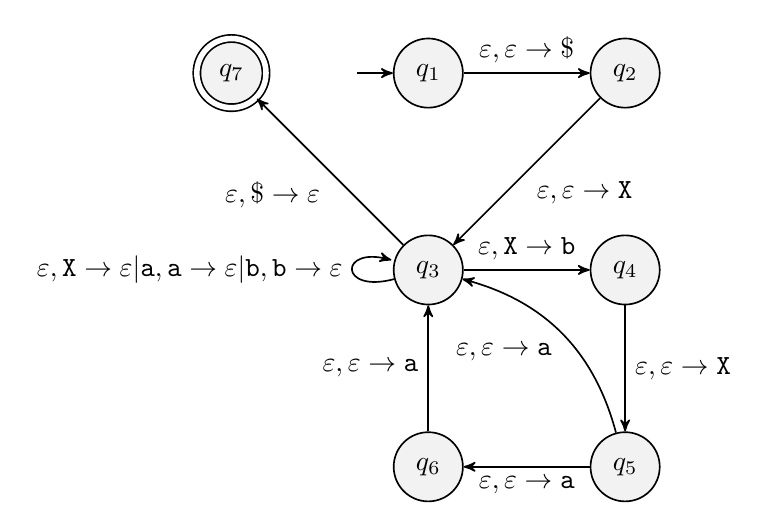
\begin{tikzpicture}
					\node[state] (q3) {$q_3$};
					\node[state, initial, above of=q3] (q1) {$q_1$};
					\node[state, right of=q1] (q2) {$q_2$};
					\node[state, right of=q3] (q4) {$q_4$};
					\node[state, below of=q4] (q5) {$q_5$};
					\node[state, below of=q3] (q6) {$q_6$};
					\node[state, accepting, left of=q1] (q7) {$q_7$};

					\draw (q1) edge node {$\varepsilon,\tt\varepsilon\to \$$} (q2);
					\draw (q2) edge node {$\varepsilon,\tt\varepsilon\to X$} (q3);

					\draw (q3) edge node {$\varepsilon,\tt X\to b$} (q4);
					\draw (q4) edge node {$\varepsilon,\tt\varepsilon\to X$} (q5);
					\draw (q5) edge node {$\varepsilon,\tt\varepsilon\to a$} (q6);

					\draw (q5) edge[bend right] node {$\varepsilon,\tt\varepsilon\to a$} (q3);
					\draw (q6) edge node {$\varepsilon,\tt\varepsilon\to a$} (q3);

					% \draw (q3) edge[loop above] node {\(\varepsilon,\tt X\to \varepsilon|a,\tt a\to \varepsilon|b,\tt b\to \varepsilon\)} (q3);
					\draw (q3) edge[loop left] node {\(\varepsilon,\tt X\to \varepsilon|a,\tt a\to \varepsilon|b,\tt b\to \varepsilon\)} (q3);

					\draw (q3) edge node {$\varepsilon,\tt\$\to \varepsilon$} (q7);
				\end{tikzpicture}
			\end{center}
		\end{solution}
	\end{parts}

	\break

	\question Consider the grammar containing the following productions.
	\begin{align*}
		S \longrightarrow & \; XaY                      \\
		X \longrightarrow & \; aX \mid \epsilon         \\
		Y \longrightarrow & \; aY \mid bY \mid \epsilon
	\end{align*}

	\begin{parts}
		\part[5] Give a formal definition, e.g. see the description of $L_1$ in Problem \ref{q:lang}, of the language generated by this grammar.
		\begin{solution}
			\[L(G)=\{a^ib^ja^k|i > 0, j,k \ge 0\}\]
		\end{solution}

		\part[5] Draw the parse tree under this grammar for the string: aaaba.
		\begin{solution}
			\begin{center}
				\begin{forest}
					for tree={
					where n children=0{tier=terminal}{},
					parent anchor=south,
					child anchor=north,
					}
					[S [X [a] [X [a] [X [\(\varepsilon\)]]]] [a] [Y [b] [Y [a] [Y [\(\varepsilon\)]]]]]
				\end{forest}
			\end{center}
		\end{solution}
		\part[5] Argue whether this grammar is ambiguous.
		\begin{solution}
			Another derivation of the string \(aaaba\),
			\begin{center}
				\begin{forest}
					for tree={
					where n children=0{tier=terminal}{},
					parent anchor=south,
					child anchor=north,
					}
					[S [X [a] [X [\(\varepsilon\)]]] [a] [Y [a] [Y [b] [Y [a] [Y [\(\varepsilon\)]]]]]]
				\end{forest}
			\end{center}
			There exist to different left most derivation for the string \(aaaba\), hence the grammar is ambiguous.
		\end{solution}
	\end{parts}
	See \href{https://tex.stackexchange.com/a/214657/44301}{this post} on using the \texttt{forest} package to draw a parse tree.

	\question Given $L_2 = \{0^i1^j2^k \mid \hspace{1mm} i,j,k \geq 0, i \neq 1 \text{ or } j = k\}$, show that
	\begin{parts}
		\part[5] $L_2$ is not regular.
		\begin{solution} 
			\\\href{https://www.geeksforgeeks.org/basic-theorems-in-toc-myhill-nerode-theorem/}{Indistinguishability:} Given a language $L$ and $x,y$ are string over $\Sigma^{*}$ , if for every string $z \in \Sigma^{*}$, $xz, yz \in L$ or $xz, yz \not\in L$ then $x$ and $y$ are said to be indistinguishable over language $L$. Formally, we denote that $x$ and $y$ are indistinguishable over $L$ by the following notation  $x R_L y$.  $R_L$ is an equivalence relation over $\Sigma^{*}$ .
			\\\href{https://www.geeksforgeeks.org/basic-theorems-in-toc-myhill-nerode-theorem/}{Myhill nerode theorem:}  A language is regular if and only if $R_L$ partitions $\Sigma^{*}$ into finitely many equivalence classes. If $R_L$ partitions $\Sigma^{*}$  into $n$ equivalence classes, then a minimal DFA recognizing $L$ has exactly $n$ states. 
			\\(Source: \href{https://www.geeksforgeeks.org/basic-theorems-in-toc-myhill-nerode-theorem/}{https://www.geeksforgeeks.org/basic-theorems-in-toc-myhill-nerode-theorem/}) 
			\\We show that $R_{L_2}$ partitions $\Sigma^{*}$ in infinite equivalence classes.
			\\Let $01^{x},01^{y} \in  \Sigma^{*}, \; \forall x,y\in \mathbb{N}, \;s.t.\; x \neq y$, then the string $2^x$ distinguish $01^{x}$ and $01^{y}$, as $01^{x}2^{x} \in L_2$ but $01^{y}2^{x} \not\in L_2$. 
\\Then this partitions $L_2$ into infinite equivalence classes.
\\So from Myhill nerode theorem $L_2$ is not regular.
\end{solution}

		\part[5] The pumping lemma for regular languages applies to $L_2$. That is, show that there is some $p$ such that if $s\in L_2$ and $|s| > p$, then $s$ can be written as $xyz$ where $|y| > 0, |xy| \leq p$, and for each $i \geq 0, xy^iz \in L$.\\
		\begin{solution}
			\\Let $p = 1$, then for any string $s = 0^a1^b2^c \in L_2$, then let $y$ be the first non empty character of $s$, $x = \epsilon$ and $z$ be the rest of the string.
			\\Now if $a>0$  then $y = 0$, then as we know $s \in L_2$, $xy^iz = 0^i 0^{a-1}1^b2^c$, and as $0^{a}1^b2^c \in L_2$ then $0^i 0^{a-1}1^b2^c \in L_2$.
			\\If $a=0$  then for  $s = 0^01^b2^c = 1^b2^c$, we have either $b>0$ then $y = 1$, then as we know $s \in L_2$, $xy^iz = 1^i 1^{b-1}2^c$, and as $1^b2^c \in L_2$ then $1^i 1^{b-1}2^c \in L_2$, or if $b=0$  then for  $s =  0^a1^b2^c  =  0^01^02^c = 2^c$, $y = 2$ then as we know $s \in L_2$, $xy^iz = 2^i2^{c-1}$, and as $2^c \in L_2$ then $2^i2^{c-1}\in L_2$. 
\\Therefore $L_2$ satisfy the pumping lemma.
		\end{solution}
	\end{parts}
	\textit{Note: This shows that the converse of the pumping lemma is false.}

	\question Our book defines a PDA, $P$, to accept a string by final state. Let $FS(P)$ denote the set of all strings accepted by $P$ by final state. Acceptance can also be defined through empty stack. That is, a string, $w$, is accepted if the stack is empty when the head has read $w$ from the tape. Let $ES(P)$ denote the set of all strings that are accepted by $P$ through empty stack.
	\begin{parts}
		\part[5] Provide a definition of acceptance by empty stack similar to the definition of acceptance by final state on Page 114 of the book. Take care that $\epsilon$ is not automatically accepted.
		\begin{solution}
			A PDA $P = (Q,\Sigma,\Gamma,\delta, q_0, F)$ accepts a string $w = w_1w_2...w_n$ where each $w_i \in \Sigma_{\epsilon}^{*}$ for $1\leq i \leq n$, if there exists a sequence of states $r_0,r_1,...,r_n \in Q$ and sequence of string $s_0,s_1,...,s_n \in \Gamma_{\epsilon}^{*}$ where each $s_j$ represent a stack condition, for $0\leq j \leq n$, such that
			\\  $r_0 = q_0$ and $s_0 = \epsilon$,
			\\ For $i = 0, ... , n-1$,  we have $(r_{i+1},b) \in \delta(r_i, w_{i+1}, a)$, where $s_i = at$ and $s_{i+1} = bt$ for some $a, b \in \Gamma_{\epsilon}$ and $t \in \Gamma_{\epsilon}^{*}$, and
			\\ $s_n = \epsilon$
			\\So we just modified the definition of acceptance of a PDA given on page 114 of the book to make the final condition of the stack to be empty for a string to be accepted ($s_n = \epsilon$).
		\end{solution}

		\part[5] Given a PDA, $P$, provide a PDA, $P_{stack}$, such that $ES(P_{stack}) = FS(P)$.
		\begin{solution}
			Let $P =  (Q,\Sigma,\Gamma,\delta, q_0, F)$ be a PDA .
			\\We construct  $P_{stack} = (Q,\Sigma,\Gamma,\delta', q_0, F)$ such that $ES(P_{stack}) = FS(P)$.
			\\ Notice that the that set of states, input alphabets, stack alphabets, start state and accept state of $P_{stack}$ and $P$ are the same, but we change the transition function. We define $\delta'$ with additional transition for every accept state, where if $\epsilon$ is input, and the stack is not empty then pop the stack, formally,
			\[\delta'(q,w,a)\begin{cases} \delta(q,w,a)& \mbox{if } q \not\in F \mbox{ or } w \neq \epsilon \\ \delta(q,w,a) \cup \{(q,\epsilon)\}& \mbox{if } q \in F \mbox{ and } w =\epsilon\end{cases}\]
			So $P_{stack}$ just pops the entire stack in an alternative branch of computation once you reach the an accept state, or thatb is to say once you reach an accept state $P_{stack}$ pops the entire stack so that the stack becomes empty. 
			\\Therefore $P_{stack}$ and  $P$ recognize the same language, so $ES(P_{stack}) = FS(P)$.
		\end{solution}

		\part[5] Given a PDA, $P$, provide a PDA, $P_{state}$, such that $FS(P_{state}) = ES(P)$.
		\begin{solution}
			Let  $P_{stack} = (Q,\Sigma,\Gamma,\delta', q_0, F)$
			\\We construct  $P = (Q,\Sigma,\Gamma,\delta, q_0, F)$ such that $ES(P_{stack}) = FS(P)$.
			\\As our construction above  in part b we are just popping the stack when we finish reading the input and we are at the accept state, so we do end in the accept state of the PDA just added that now the stack will also be empty. Therefore for the PDA $P_{stack}$ the same PDA will have $ES(P_{stack}) = FS(P_{stack})$, therefore $P_{stack} = P$. 
			\\Therefore $P_{stack}$ and  $P$ recognize the same language, so $ES(P_{stack}) = FS(P)$.
		\end{solution}
	\end{parts}
\end{questions}

\end{document}

%%% Local Variables:
%%% mode: latex
%%% TeX-master: t
%%% End:
